% !TeX root = ../index.tex

\section{Bestandteile der Hardwareschicht}

Wie bereits im vorherigen Kapitel angedeutet bildet die Hardwareschicht den untersten Baustein der Systemarchitektur. In diesem Kapitel werden die Methoden vorgestellt, die während des Laborprojekts eingesetzt wurden, um mit der Hardware arbeiten zu können. Desweiteren werden die einzelnen Hardwarebestandteile aufgedrosselt und deren Funktionsweise näher beschrieben.

Beim Arbeiten mit der eingesetzten Hardware haben wir auf die browserbasierte Anwendung Wokwi gesetzt, welche über den Link \textit{https://wokwi.com} erreichbar ist. Die Entscheidung für die virtuelle Umgebung Wokwi wurde aus dem Grund getroffen, da das Aufbauen einer Netzwerkumgebung im Labor nicht möglich ohne Weiteres war. Die Simulation in Wokwi kann allerdings im Anschluss auf die reale Welt übertragen werden und der entwickelte Code läuft auf den entsprechenden Hardwaregeräten ohne eine notwendige Konvertierung.

Bezüglich der eingesetzten Hardware kommen bei unserer intelligenten Gartenbewässerung insgesamt zwei ESP32-Mikrocontroller des Unternehmens Espressif Systems zum Einsatz. Mithilfe der Mikrocontroller können die angeschlossenen Sensoren und Aktoren angesteuert werden. Dabei wird ein ESP32-Mikrocontroller für die Sensoren und einer für die Aktoren eingesetzt. Im folgenden werden vorerst die Sensoren und anschließend die Aktoren näher beleuchtet.

\subsection{Einsatz von Sensoren}
Als Temperatur- und Feuchtigkeitssensor setzen wir in der virtuellen Wokwi Umgebung auf einen DHT22 Sensor. Insgesamt setzen wir davon zwei Stück ein, einen für die Werte in der Luft und einen für die Werte im Boden bzw. in Bodennähe.

In der realen Welt ist der DHT22 Sensor allerdings für die Messung der Bodenfeuchtigkeit nicht geeignet. Grund dafür ist, dass der DHT22 Sensor nicht wasserresistent ist. Im realen Anwendungsfall würde sich ein kapazitiver Bodenfeuchtesensor des Herstellers AZDelivery für die Ermittlung der Feuchtigkeitswerte im Boden anbieten. Die Messsonde wird in den Boden gesteckt und es wird die Feuchtigkeit des Bodens anhand von Veränderungen in der Kapazität gemessen. Ein solcher Sensor verfügt über einen integrierten Verstärker und kann direkt an einen analogen Eingang eines ESP angeschlossen werden. \newline
Für die Messung der Lufttemperatur sollte ebenso bedacht werden, dass der Sensor nicht direktem Niederschlag als auch direkter Sonneneinstrahlung ausgesetzt ist. Entsprechend sollte ein Schutz bzw. eine Umhüllung um den DHT22 Sensor ergänzt werden. Wichtig ist jedoch, dass die Luft weiterhin frei innerhalb des Schutzes zirkulieren kann, um präzise Sensorwerte zu erhalten.\newline
In der Wokwi Umgebung gibt es allerdings nur eine begrenzte Auswahl an Hardwaresensorik. In Wokwi steht der zweite DHT22 Sensor somit für die oberflächennahe Temperatur des Bodens und repräsentativ für die Feuchtigkeit im Boden. Die Werte, die der DHT22 Sensor liefert, werden zum einen in Grad Celsius und zum anderen in Prozent angegeben.

Für die Ermittlung der Helligkeit wird ein LDR-Fotowiderstand Sensor eingesetzt, welcher die Stärke der Sonneneinstrahlung erfasst. Bei dem Umgang bezüglich der Einheit der vom LDR Sensor gelieferten Werte haben sich ein paar Schwierigkeiten aufgetan. Der LDR Sensor liefert auf dem digitalen Output-Pin Werte im Bereich von '0' bis '65535'. Der Wert steigt dabei, wenn die Sonneneinstrahlung schwächer wird, und sinkt, wenn es in der Umgebung heller wird. Der Wert ergibt sich dabei aus dem Widerstand des Sensors und der Spannung, die am Sensor anliegt. Auf die interne Funktionsweise des Sensors wird allerdings im Rahmen dieses Laborberichts nicht weiter eingegangen. Die Herausforderung liegt nun dabei, den gelieferten Wert am digitalen Output-Pin in die Einheit Lux umzurechnen, um damit in der weiteren Entwicklungsarbeit Logiken definieren zu können. In List. \ref{list:LDR_Berechnung} ist ein MicroPython-Ausschnitt dargestellt, der den Wert des LDR Sensors in die Einheit Lux umrechnet.


\begin{listing}[!ht]
\begin{minted}{python3}
ldr_digital_value = ldr.read_u16()
# Convert digital value to lux
ldr_voltage = ldr_digital_value / 65535 * 5
ldr_resistance = 2000 * ldr_voltage / (1 - ldr_voltage / 5)
brightness_value = 
    round(pow(LDR_RL10 * 1e3 * pow(10, LDR_GAMMA) / ldr_resistance, 
        (1 / LDR_GAMMA)))
\end{minted}
\caption{Berechnung des Lux-Wertes aus dem LDR-Fotowiderstand}
\label{list:LDR_Berechnung}
\end{listing}
    

Die drei oben aufgeführten Sensoren werden an einen ESP32-Mikrocontroller angeschlossen, welcher mit dem hausinternen \gls{wlan} verbunden ist. Abb. \ref{fig:wokwi_sensoren} zeigt nochmals zusammenfassend einen visuellen Auszug aus Wokwi, auf dem der Anschluss der Sensorik an den ESP32-Mikrocontroller dargestellt ist. Auf der rechten Seite befinden sich die beiden DHT22 Sensoren, auf der linken Seite der LDR-Fotowiderstand Sensor und in der Mitte der ESP32-Mikrocontroller.

\begin{figure}[h]
    \centering
    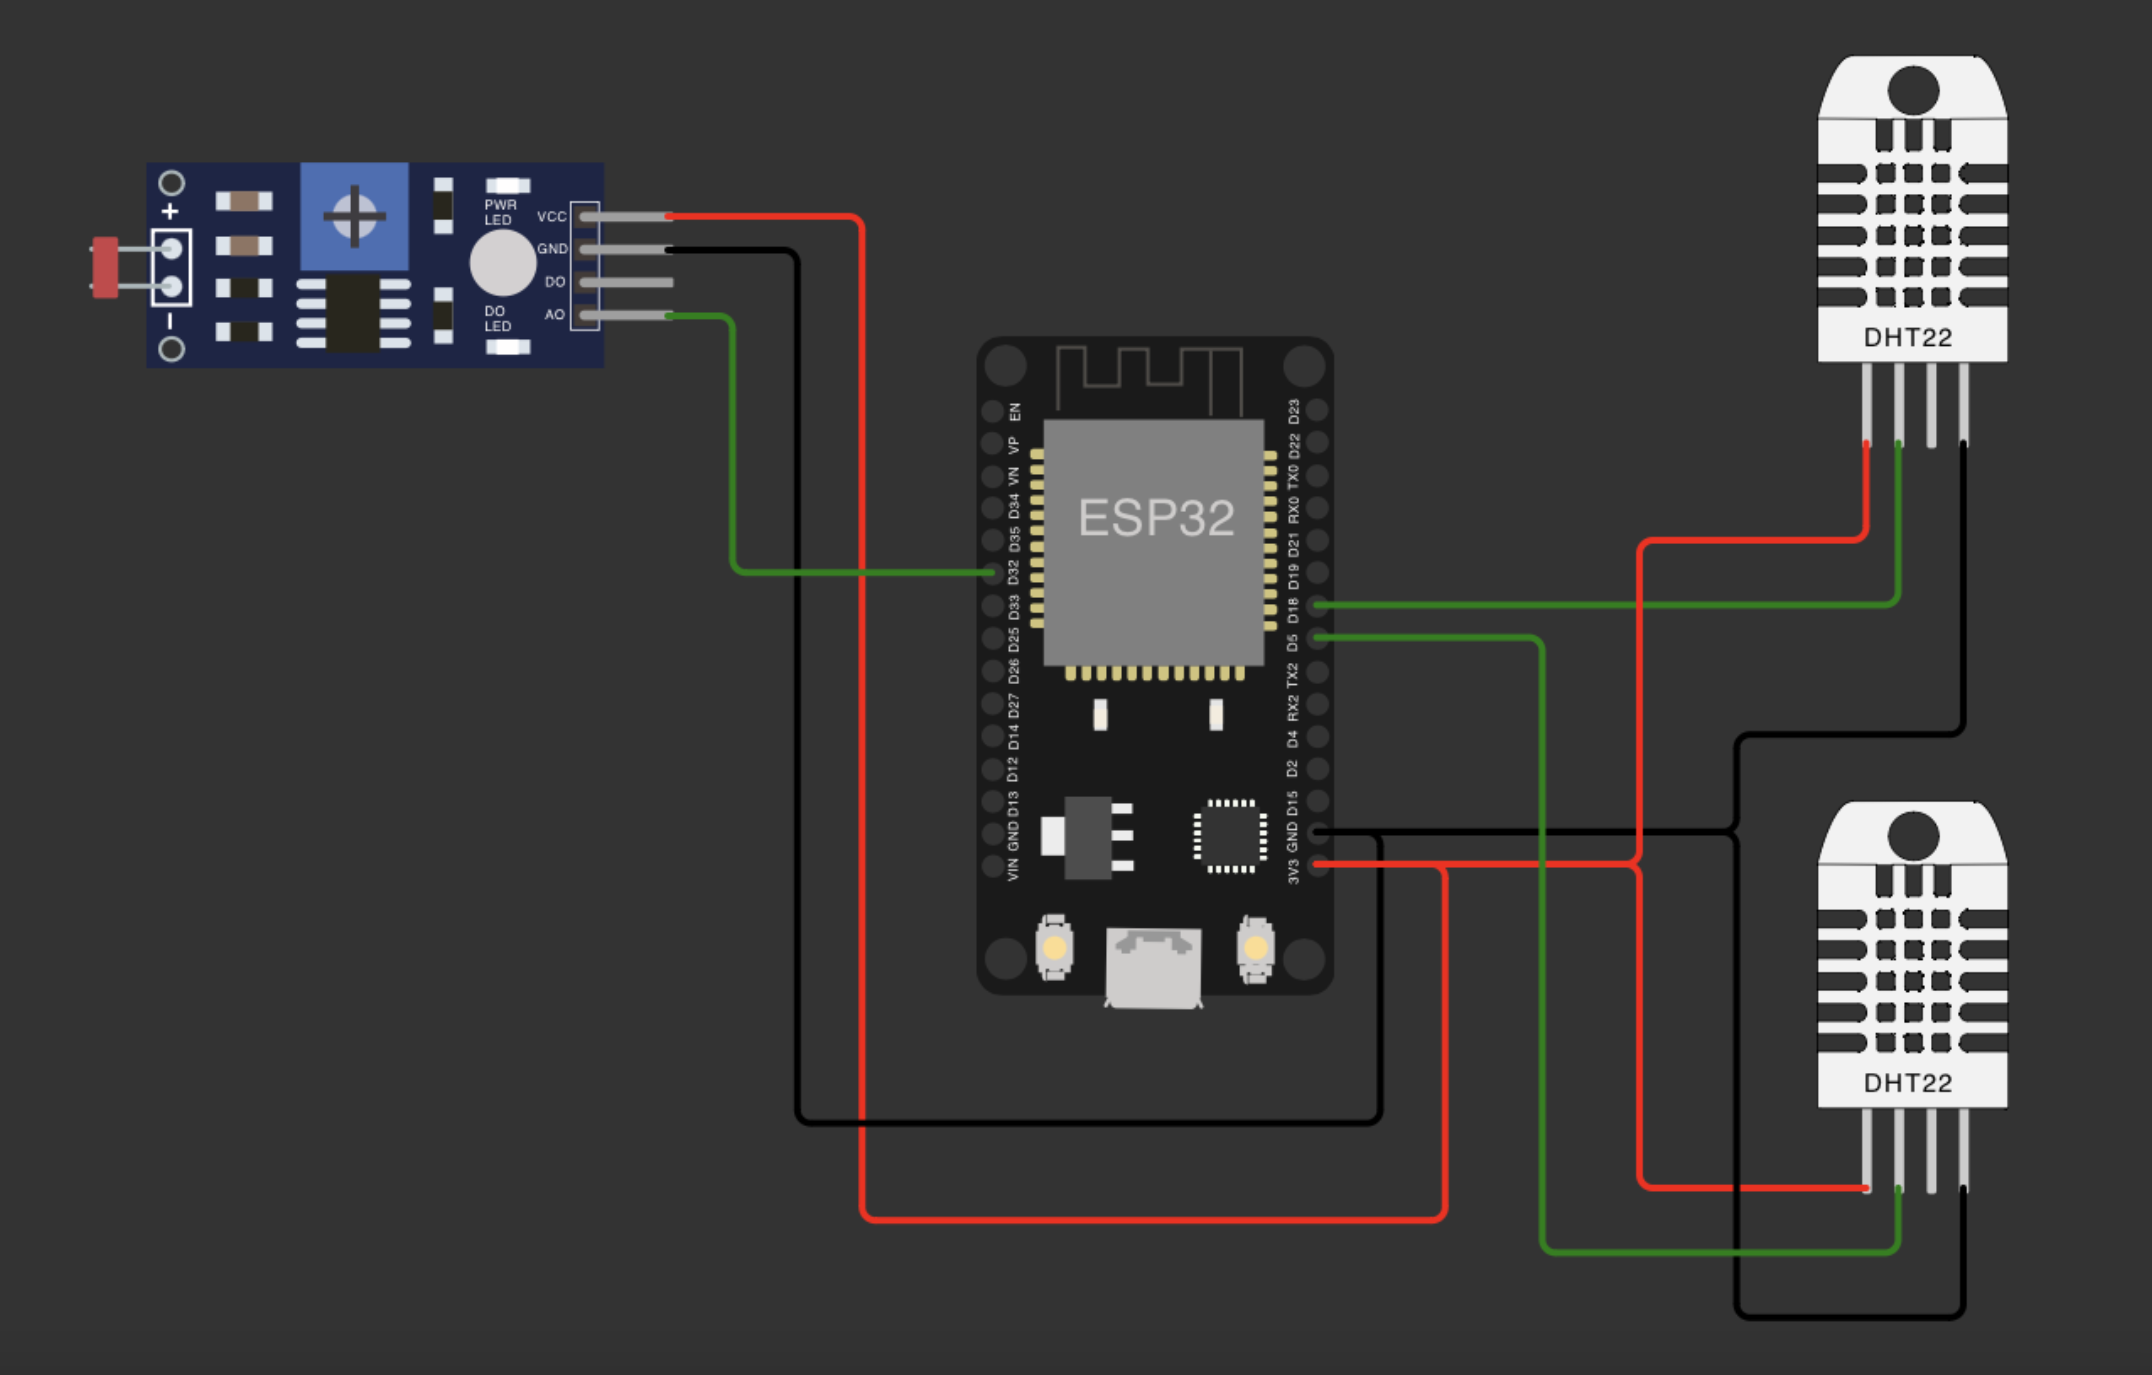
\includegraphics[width=0.8\textwidth]{Wokwi_Sensoren.png}
    \caption{Anschluss der Sensorhardware in der virtuellen Umgebung Wokwi}\label{fig:wokwi_sensoren}
\end{figure}

\subsection{Einsatz von Aktoren}
Bezüglich der Steuerung der Markise, um die Sonneneinstrahlung zu reduzieren, verwenden wir einen Servo-Motor, der die Markise aus- und einfahren kann. Die Steuerung des Servo-Motors läuft über die MicroPython Library \textit{Servo}. Über die Angabe eines Winkels bewegt sich der Servo-Motor in die gewünschte Position. Somit kann die Markise über die Drehung des Motors um einen bestimmten Winkel ein- bzw. ausgefahren werden.

Die Steuerung der Wasserpumpe übernimmt ein Relais, welches durch das Schalten eines neuen Stromkreises die Wasserpumpe an- bzw. ausschalten kann. In MicroPython definieren die Werte '0' und '1' des Relais, ob der Stromkreis geschlossen oder offen ist. In Wokwi haben wir zu Demonstrationszwecken eine LED an das Relais angeschlossen, um zu veranschaulichen, ob die Wasserpumpe läuft oder nicht. Im realen Anwendungsfall wird an das Relais anstatt der Wokwi-LED eine Wasserpumpe angeschlossen.

Die beiden Aktoren Servo-Motor und Relais sind an einen ESP32-Mikrocontroller angeschlossen, welcher zusammen mit dem Mikrocontroller der Sensoren mit dem hausinternen \gls{wlan} verbunden ist. Abb. \ref{fig:wokwi_aktoren} zeigt nochmals, analog zum vorherigen Unterkapitel, einen Ausschnitt aus Wokwi, auf dem die Verkabelung der Aktoren mit dem ESP32-Mikrocontroller dargestellt ist. Am oberen Bildrand befindet sich der Servo-Motor, am unteren Bildrand das Relais mit angeschlossener LED und links der ESP32-Mikrocontroller. Im Anhang in List. \ref{list:wokwi_aktoren1}ff. findet sich der Quellcode zu der Python-Implementierung für diesen ESP.

\begin{figure}[h]
    \centering
    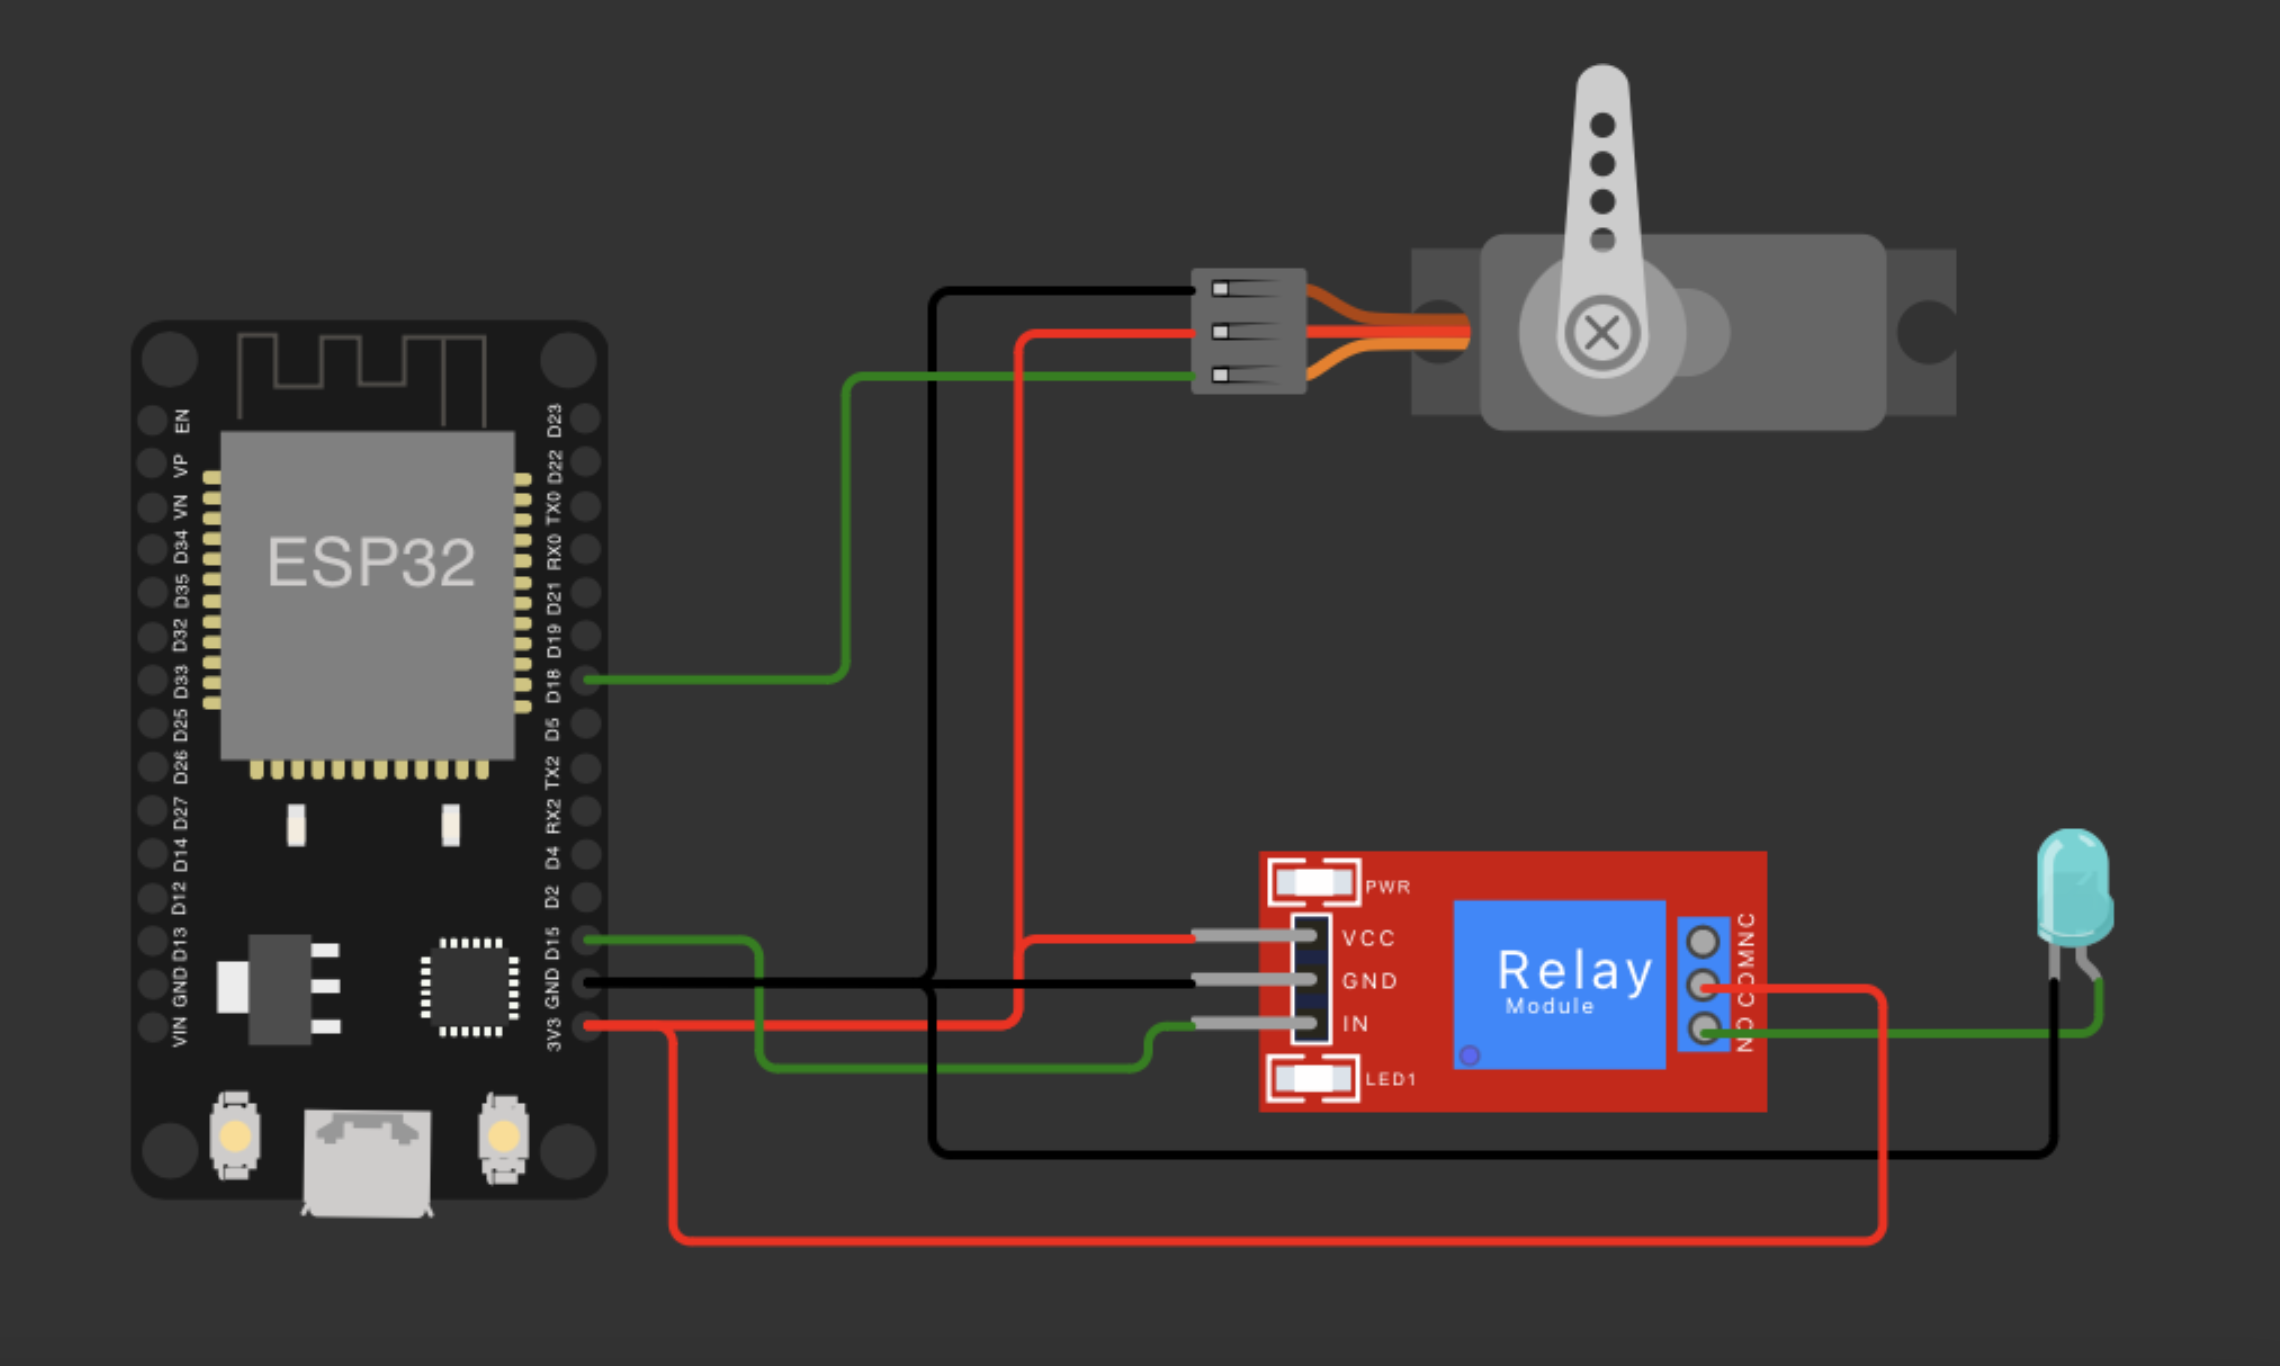
\includegraphics[width=0.8\textwidth]{Wokwi_Aktoren.png}
    \caption{Anschluss der Aktorenhardware in der virtuellen Umgebung Wokwi}\label{fig:wokwi_aktoren}
\end{figure}